\documentclass[12pt,a4paper]{article}
% \usepackage[english]{babel}
% \usepackage[utf8x]{inputenc}

\usepackage{graphicx} % Required for inserting images.
\usepackage[margin=25mm]{geometry}
\parskip 4.2pt  % Sets spacing between paragraphs.
% \renewcommand{\baselinestretch}{1.5}  % Uncomment for 1.5 spacing between lines.
\parindent 8.4pt  % Sets leading space for paragraphs.
\usepackage[font=sf]{caption} % Changes font of captions.

\usepackage{amsmath}
\usepackage{amsfonts}
\usepackage{amssymb}
\usepackage{siunitx}
\usepackage{verbatim}
\usepackage{hyperref} % Required for inserting clickable links.
\usepackage{natbib} % Required for APA-style citations.
\usepackage{fancyhdr}

\title{CREATE Protocol : Decentralised Ownership \\ for the 100x AI-first Creator}
\author{\href{https://orcid.org/0000-0001-5431-6367}{\hspace{1mm}Dipankar Sarkar} \\
  \texttt{me@dipankar.name} \\
        \and
	Abhishek Krishna \\
	%% Address \\
	\texttt{abhishek@createprotocol.org} \\
	%% \And
	%% Coauthor \\
	%% Affiliation \\
	%% Address \\
	%% \texttt{email} \\
	%% \And
	%% Coauthor \\
	%% Affiliation \\
	%% Address \\
	%% \texttt{email} \\
 }


\begin{document}
\pagestyle{fancy}
%... then configure it.
\fancyhead{} % clear all header fields
\fancyhead[RO,LE]{\textbf{CREATE Protocol}}
\fancyfoot{} % clear all footer fields
\fancyfoot[LE,RO]{\thepage}
\fancyfoot[LO,CE]{}
\fancyfoot[CO,RE]{}

\maketitle

\begin{abstract}
The Create protocol, poised at the forefront of the AI-driven creative revolution, introduces the groundbreaking Creative Object Model (COM), a dynamic non-fungible token system that transforms digital artistry and ownership. This whitepaper unveils a platform where AI and blockchain synergize, redefining content as a living, evolving entity. The protocol offers a novel economic model, balancing the interests of artists, consumers, and computation nodes with a sophisticated royalty system and democratic governance. Highlighting a robust technological infrastructure with advanced generative AI, decentralized storage, and user-friendly interfaces, the protocol prioritizes scalability, security, and accessibility. The roadmap ambitiously progresses from text and images to more complex media, embodying a commitment to continuous innovation. Create protocol invites creators, developers, and visionaries to join a movement that transcends traditional boundaries, magnifying their impact in the digital creative realm. This document is a manifesto for those aspiring to shape the future of digital creativity.
\end{abstract}

\pagebreak

\tableofcontents

\pagebreak

\section{Introduction}\label{sec:intro}

In the burgeoning era of artificial intelligence and decentralized technologies, the very fabric of creative expression and ownership is undergoing a radical transformation. At the forefront of this revolution stands the Create protocol, a visionary platform poised to redefine the paradigms of artistic creation and consumption in the digital age. This whitepaper presents an in-depth exploration of the Create protocol, a groundbreaking initiative that promises to usher in a new epoch of creative possibilities, powered by the synergies of AI and blockchain technology.

At its core, the Create protocol is an audacious attempt to navigate and reshape the uncharted territories of AI-driven creativity. It is a bold response to the evolving landscape where traditional notions of content ownership, copyright, and consumption are being relentlessly challenged and redefined. The advent of advanced machine learning models and generative algorithms has precipitated a seismic shift in how content is created, distributed, and experienced. In this transformative context, the Create protocol emerges as a beacon of innovation, offering a new model for creative expression that is fluid, dynamic, and deeply personalized.

The essence of the Create protocol is encapsulated in its pioneering concept of the Creative Object Model (COM) - a dynamic Non-Fungible Token (NFT) that embodies the fusion of artistic ingenuity and AI sophistication. This revolutionary model extends beyond the static consumption of content, inviting a paradigm where content is not merely viewed or heard but interacted with, remixed, and evolved. Through the COM, artists and creators are empowered to become more than just the originators of content; they metamorphose into ongoing contributors to a living, breathing artistic process, where their style, personality, and creative essence are infused into personalized and ever-evolving experiences for the consumer.

In this whitepaper, we delve into the intricate mechanics of the Create protocol, unraveling how it augments and redefines the realms of creative ownership in an AI-dominated era. We dissect the standards and analytics that underpin this new era of creative consumption, offering a thorough examination of how the protocol not only adapts to but also anticipates the future trajectories of digital creativity. The document also explores the economic and governance models intrinsic to the protocol, elucidating how they synergize to foster a sustainable and thriving ecosystem for artists, developers, and consumers alike.

As we embark on this exploration, the Create protocol stands as a testament to the limitless potential of human imagination when harmoniously aligned with the transformative power of AI. It is an invitation to venture into a future where creativity is not a finite artifact but an ever-evolving journey, a dynamic interplay between the creator and the consumer, mediated by the profound capabilities of artificial intelligence. This whitepaper is your guide to understanding and engaging with this bold new world - a world where the boundaries of creation are constantly expanding, driven by the relentless pursuit of innovation and the indomitable spirit of human creativity.
It is possible to cite multiple references at the same time.

\section{Background and Rationale}\label{sec:background}

As we stand on the brink of a new era, defined by the intersection of groundbreaking technological advancements and creative expression, it becomes imperative to understand the forces that have led us to this pivotal moment. The second chapter of our journey into the Create protocol delves into the historical context and the compelling rationale behind this revolutionary platform. It is a narrative that traverses through the evolution of creative ownership in the age of AI, illuminating the shifting paradigms that have set the stage for this monumental leap in the realm of digital creativity.

The digital age, marked by its rapid technological advancements, has always been a double-edged sword for creative expression. On one hand, it has democratized content creation and distribution, allowing artists and creators from every corner of the globe to share their work with unprecedented ease. On the other hand, it has also ushered in complexities surrounding copyright and ownership, often muddling the waters of artistic control and compensation. The emergence of sophisticated AI and machine learning technologies has only amplified these complexities, challenging the traditional frameworks of intellectual property and blurring the lines between creator and creation.

In this landscape, where AI algorithms can remix, repurpose, and regenerate content, the conventional definitions of ownership and copyright begin to crumble. What does it mean to own a piece of art when it can be algorithmically transformed into something entirely new? How do we ascribe value and rights to creations that are born out of collaborative interplays between human ingenuity and machine intelligence? These are not just philosophical musings but real questions that demand nuanced answers in today’s digital ecosystem.

The Create protocol emerges as a response to these profound questions, offering a model that not only embraces but also celebrates the dynamic nature of AI-driven creativity. It posits a future where the lines between creators, consumers, and collaborators are fluid, and where the value of creative work is not just in its original form but in its potential to evolve and adapt. This is a future where creative ownership is redefined, moving away from rigid structures to more flexible and inclusive frameworks that recognize and reward the multifaceted contributions in the creative process.


The rationale for the Create protocol is deeply rooted in the recognition of this new era of creative consumption. In this era, content is not a static entity to be consumed passively; rather, it is an active participant in an ongoing creative dialogue. This dialogue is not just between the creator and the consumer but also includes the AI algorithms that bring their own unique flavor to the creative mix. The protocol acknowledges the complexities and opportunities of this new landscape, providing a structure that harnesses the potential of AI-driven creativity while ensuring fair compensation and recognition for all contributors.

\noindent\fbox{%
    \parbox{\textwidth}{%
The Create protocol's background and justification demonstrate a thorough comprehension of the significant changes occurring in the digital creative field. It acknowledges the obstacles and possibilities that await and expresses a strong commitment to navigate these unknown territories with a forward-looking, inclusive, and innovative approach. This portion of the whitepaper establishes the foundation for a thorough examination of the protocol, providing a comprehensive grasp of its mechanisms, consequences, and potential to redefine creative expression in the digital era.
}%
}

\pagebreak

\section{New Paradigms in Creation and Consumption}\label{sec:new-paradigm}

The core of the Create protocol is centered around a revolutionary vision that questions and redefines the existing standards of artistic production and consumption. This section of the whitepaper delves into the emerging patterns that are reshaping the realm of digital creativity, driven by the progress in AI and blockchain technologies. In this context, we examine the significant consequences of these changes, highlighting how the protocol not only adjusts to but also drives a new era of vibrant and engaging content.

\subsection{The Concept of Dynamic Content Interaction}

At the vanguard of this new era is the concept of dynamic content interaction. Unlike traditional models where content is created, published, and consumed in a static form, dynamic interaction posits a fluid and ever-evolving relationship between the creator, the content, and the consumer. In this paradigm, content is not a finished product but a starting point for continuous evolution and reinterpretation.

This shift is significantly driven by Generative AI's ability to learn, adapt, and generate new content (LLMs, Diffusion Models, GANs) based on existing works. It allows for a creative process that is not linear but cyclical, where each interaction with the content can lead to new variations, influenced by the unique inputs of diverse users. The result is a living tapestry of creativity, where the boundaries between creation, modification, and consumption become increasingly blurred.


\begin{figure}[ht]
    \centering
    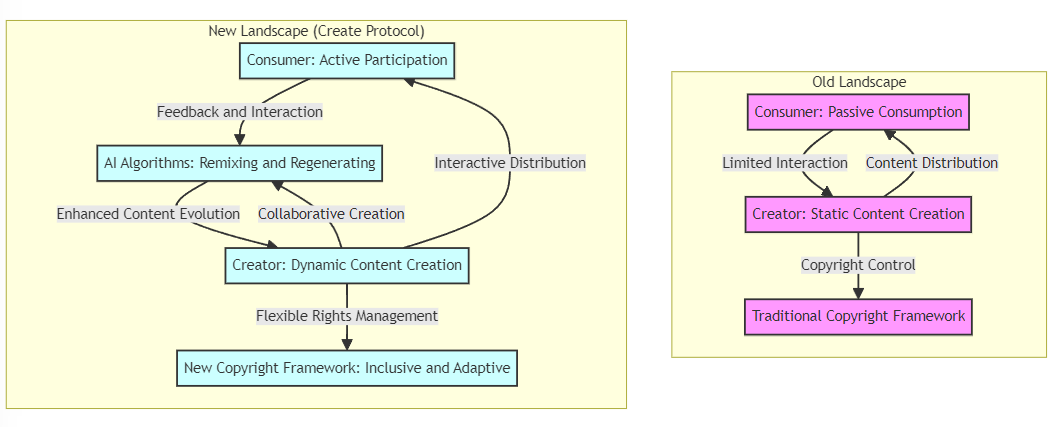
\includegraphics[width=1\linewidth]{create_1.png}
    \caption{Changing creative landscape}
    \label{fig:enter-label}
\end{figure}

\subsection{Impact of AI on Copyright and Ownership}

The rise of AI in creative processes poses complex challenges to traditional notions of copyright and intellectual property. When an AI system can analyze, learn from, and generate new content based on existing works, the lines of ownership and authorship become intertwined and often indistinct. This raises critical questions: Who owns the derivative works created by AI? How do we attribute value and rights in a landscape where human and machine creativity coalesce?

The Create protocol approaches these questions with a nuanced understanding. It recognizes that in the AI era, copyright cannot be anchored in rigid, antiquated frameworks. Instead, it advocates for a more dynamic, flexible approach that respects original creation while embracing the evolutionary nature of AI-generated content. This approach acknowledges the collaborative interplay between human creators, AI algorithms, and consumers, aiming to ensure fair recognition and compensation for all parties involved.



\subsection{The Future of Content Consumption and Creation}

The future envisioned by the Create protocol is one where content consumption and creation are part of a continuous, interactive loop. In this future, creators are not just producers of content but curators of experiences, guiding the AI as it tailors and personalizes content for individual users. Consumers, on the other hand, are not passive recipients but active participants, their interactions and preferences feeding into the AI to create bespoke experiences.

This paradigm shift extends beyond mere technology; it is a cultural and philosophical evolution in how we perceive and engage with creative works. It champions a more inclusive, participatory, and fluid model of creativity, one that breaks down barriers and fosters a collaborative ecosystem where everyone’s contribution is valued.

\noindent\fbox{%
    \parbox{\textwidth}{%
We have illuminated a future where AI-driven creativity is not a distant dream but an imminent reality. It underscores the need for a reimagined framework of creative ownership and copyright, one that is adaptable, equitable, and reflective of the dynamic interplay between human and machine intelligence. This section sets the stage for a deeper exploration of the Create protocol's mechanisms and its potential to revolutionize the way we create, consume, and interact with content in the digital age.
}%
}

\pagebreak

\section{The Creative Object Model (COM)}

In this crucial part of the whitepaper for the Create protocol, we present and analyze the fundamental aspect of our platform - the Creative Object Model (COM). This groundbreaking idea signifies a significant change in the field of digital creativity, combining the abilities of AI with the core of human artistic expression. In this section, we delve into the complexities of COM, its impact on transforming content interaction, and its consequences for creators and users in the future influenced by AI.

\subsection{Definition and Significance of COM}

The Creative Object Model (COM) is not merely a technological construct but a radical rethinking of what constitutes a digital creative work. At its heart, COM is a dynamic, AI-first Non-Fungible Token (NFT) that embodies more than just a static piece of art or media. It is a living, evolving entity that encapsulates the style, personality, and creative intellect of its originator - the artist. COMs are unique in that they are not finite creations but ongoing projects, continuously shaped and reshaped by interactions with consumers and AI algorithms.

The importance of COM lies in its capacity to change the dynamic between the creator and the consumer. In the conventional model, this dynamic is transactional - the creator produces content, and the consumer passively receives it. COM disrupts this model by allowing for an interactive, fluid exchange where content is personalized with the artist's style and adapts based on user interactions, with generative AI.

\subsection{Dynamic NFTs and Personalized Creative Experiences}

Dynamic NFTs, as embodied by COMs, are a breakthrough in personalizing creative experiences. Unlike conventional NFTs, which represent static ownership of a digital asset, dynamic NFTs are fluid and responsive. They allow consumers to not just own a piece of art but to engage with it, influence its evolution, and experience it in a way that is tailored to their preferences and interactions.

This dynamic nature of COMs opens up new avenues for creators. Artists can now extend their creative expression beyond the initial act of creation, continuously influencing how their work evolves and interacts with its audience. It transforms the artist from a creator of content into a provider of creative services, where their artistic style and vision can be applied in varied and personalized contexts.

\begin{figure}
    \centering
    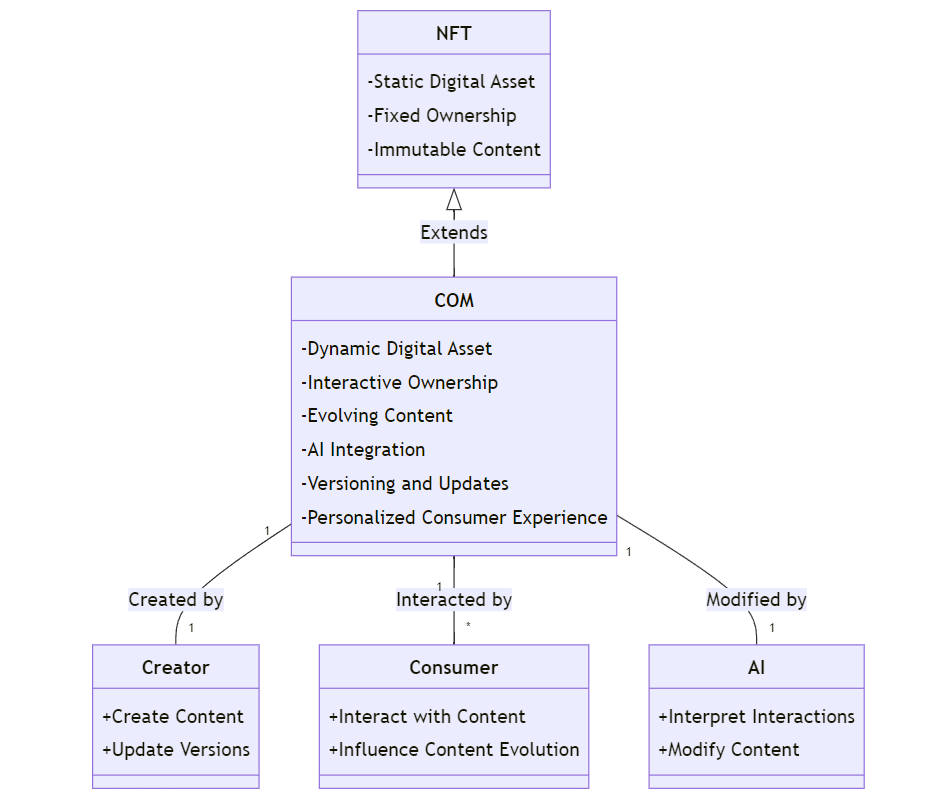
\includegraphics[width=0.8\linewidth]{create_2.png}
    \caption{COM draft architecture}
    \label{fig:com-architecture}
\end{figure}

\subsection{Versioning and Artist-Specific Updates}

A key feature of the COM framework is its support for versioning and artist-specific updates. This feature ensures that a COM is not a static entity but a canvas for ongoing creative expression. Artists can update their COMs, either to reflect their evolving style or to respond to consumer interactions and feedback. This creates a living digital asset that not only retains its value over time but potentially increases in value as it grows and evolves with the artist's career.

\subsection{The Economic Model: From Creation to Consumption}

The economic model underpinning COMs is as innovative as their technology. It shifts the focus from the sale of a single, static piece of content to a more dynamic, engagement-based model. Creators can monetize their work through initial sales, but also through ongoing interactions and personalizations facilitated by the COM. Consumers, in turn, invest not just in a piece of content, but in a creative journey that offers them a personalized and ever-evolving experience.

\subsection{The Role of AI in COM}

AI plays a central role in the functionality of COMs. It acts as the intermediary that interprets user interactions and translates them into creative modifications and evolutions of the COM. This AI-driven process ensures that each COM is not just a reflection of the original artist's vision, but also a product of the continuous interplay between the creator, the consumer, and the AI.

\noindent\fbox{%
    \parbox{\textwidth}{%
In summary, the whitepaper's section on the "Creative Object Model (COM)" delves deeply into the fundamental aspects of the Create protocol. It presents a vision of a future where digital creativity is not confined to a single occurrence but rather an ongoing and interactive process. The COM represents this vision by demonstrating how AI can enrich and personalize the creative journey, while also introducing a new economic model for digital artists. This section lays the foundation for understanding how the Create protocol employs technology to forge a new path in the realm of digital art and creativity.
}%
}

\section{Economic Model and Royalties}

In this part of the Create protocol whitepaper, we explore the complex economic model that forms the foundation of the system. The emphasis is on the methods of distributing royalties and analyzing the game-theoretic interactions among different stakeholders in the ecosystem. The economic structure of the protocol is carefully designed to motivate and harmonize the interests of artists, consumers, computation nodes, and other participants, with the ultimate goal of establishing a sustainable and flourishing creative economy.

\subsection{Understanding the COM Royalty Formula}

At the core of the Create protocol's economic model is the COM Royalty Formula, a sophisticated mechanism designed to fairly distribute earnings generated from the dynamic interactions of COMs. This formula accounts for various factors such as the original creator's input dataset, the degree of transformation or personalization by AI as this might be used in conjunction with other COMs, and the consumer's interaction level. The royalty system is structured to ensure that creators are continuously compensated for their work, reflecting the evolving nature of their creations and the ongoing engagement they foster.

\subsection{\$CREATE: The Native Token of the Create Protocol}

The \$CREATE token plays a crucial role in the economy of the Create protocol. It acts as a means of exchange, facilitating various transactions within the ecosystem, including the acquisition of COMs, payment for AI services, and rewarding computation nodes. The tokenomics of \$CREATE are carefully designed to uphold a stable economy, preventing inflation and ensuring that the token's worth is linked to the actual utility and demand within the ecosystem.

\begin{figure}
    \centering
    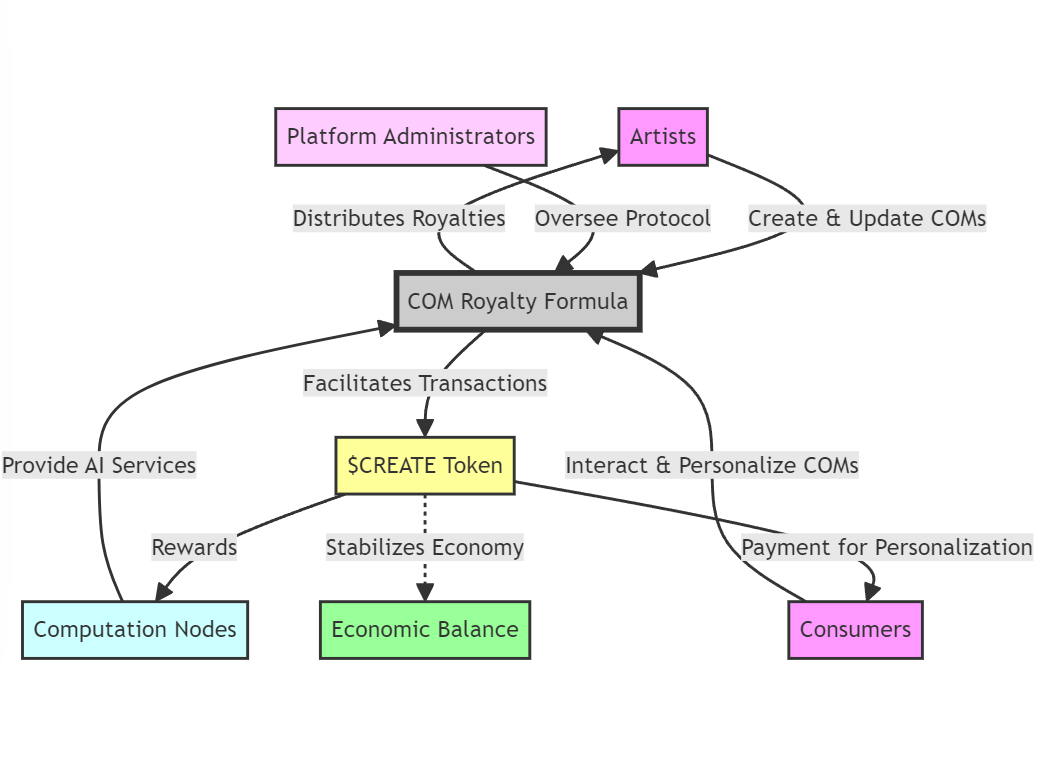
\includegraphics[width=0.8\linewidth]{create_3.png}
    \caption{High-level economic cycle}
    \label{fig:economic-cycle}
\end{figure}

\subsection{Game Theoretic Analysis of Stakeholder Interactions}

The analysis of the Create protocol from a game theoretic perspective examines the strategic interactions between different stakeholders involved, namely artists, consumers, computation nodes, and platform administrators. Each participant in the system possesses unique motivations and incentives.

\begin{itemize}
    \item \textbf{Artists} are motivated by creative expression and economic gain. They seek to maximize their earnings through the creation and continuous updating of COMs, balancing the need for artistic integrity with market demand.
    \item \textbf{Consumers} desire personalized, evolving content. Their interactions with COMs are driven by the utility they derive from personalized experiences, and they are willing to pay for higher levels of personalization and uniqueness.
    \item \textbf{Computation Nodes} provide the necessary infrastructure for the AI-driven personalization of COMs. Their incentive is to maximize the utilization of their computational resources and earn \$CREATE tokens in return for their services.
    \item \textbf{Platform Administrator}s oversee the protocol's overall health and evolution. They are incentivized to maintain a balanced and growing ecosystem, ensuring the protocol adapts to changing market dynamics and technological advancements.
\end{itemize}

The equilibrium in this system is achieved when the interests of all parties are aligned, leading to a sustainable and flourishing creative economy. The protocol's design encourages cooperation and fair competition, ensuring that no single stakeholder can monopolize the system to the detriment of others.

\subsection{Economic Incentives for Creation and Consumption}

The economic model of the Create protocol is structured to provide clear incentives for both creation and consumption. Artists are incentivized to create and update COMs, as they receive ongoing royalties and can capitalize on their evolving creative reputation. Consumers are incentivized to engage with and personalize COMs, as they receive personalized, unique experiences. This symbiotic relationship ensures a dynamic market where the value of creative works is continually enhanced through interaction and personalization.

\subsection{Long-Term Sustainability and Growth}

The long-term sustainability and growth of the Create protocol's economy are ensured through a careful balance of supply and demand, as well as continuous adaptation to market trends and technological advancements. The protocol incorporates feedback and adaptation mechanisms, allowing it to evolve with the changing landscape of AI-driven creativity.

\noindent\fbox{%
    \parbox{\textwidth}{%
To summarize, the "Economic Model and Royalties" section of the whitepaper discusses a detailed and fair economic system that supports the Create protocol. It provides a deep understanding of the motivations and relationships among various participants in the ecosystem. By applying game-theoretic principles, the economic model is designed to encourage continuous participation, innovation, and expansion. This economic framework plays a crucial role in the protocol's goal of transforming the digital creative economy.
}%
}

\pagebreak

\section{Technology and Infrastructure}

This critical section of the Create protocol whitepaper explores the sophisticated technological infrastructure and innovative solutions at the foundation of the protocol. It underscores how cutting-edge technology and robust infrastructure are harmoniously integrated to support the dynamic and complex ecosystem of the Create protocol, facilitating the creation, distribution, and consumption of COMs (Creative Object Models).

\subsection{AI-First Approach and Dynamic Object Model}

The central aspect of the Create protocol is its main emphasis on generative AI, which employs advanced algorithms to facilitate model refinement and combined inference in order to support the dynamic nature of COMs. This approach involves utilizing QLora finetuning for LLMs and Diffusion Models. This dynamic capability, powered by AI, is what sets COMs apart, transforming them from fixed digital assets into constantly evolving entities.

\subsection{Decentralized Training and Inference Mechanisms}

Decentralized computation mechanisms form the core of the Create protocol's infrastructure. These mechanisms enable the distributed processing of fine-tuning and inference tasks, ensuring efficient handling of the computation needed for personalizing and evolving COMs across multiple nodes. This decentralization improves the scalability and resilience of the system, while also promoting the inclusion of computation nodes and creating a more fair and robust network.


\subsection{Model Weight Storage on IPFS}

The InterPlanetary File System (IPFS) is used to handle the storage of both base model weights and finetuned weights. IPFS is a decentralized storage solution that guarantees the security, immutability, and accessibility of the model data used in the creation of the COM object. This decentralized approach provides improved security and transparency, as well as ensures that the data cannot be tampered with and is always available for verification and auditing purposes.

\subsection{The Role of Blockchain in Securing Transactions and Ownership}

The Create protocol heavily relies on blockchain technology to ensure the security of transactions and establish a transparent ownership system. By utilizing blockchain, the protocol is able to maintain an unchangeable record of transactions, including the creation, sale, and transfer of COMs. This feature guarantees the integrity and traceability of all activities within the ecosystem, ultimately building trust and reliability among users.


\subsection{Building a User-Friendly UI and developer-first SDK}

Recognizing the importance of accessibility and ease of use, the Create protocol prioritizes the development of a user-friendly interface (UI) and a comprehensive Software Development Kit (SDK). The UI is designed to be intuitive and engaging, catering to both seasoned creators and novices in the digital creative space. The SDK, on the other hand, provides developers with the tools and frameworks necessary to build applications and services that interact seamlessly with the Create protocol, fostering innovation and expansion of the ecosystem.


\begin{figure}
    \centering
    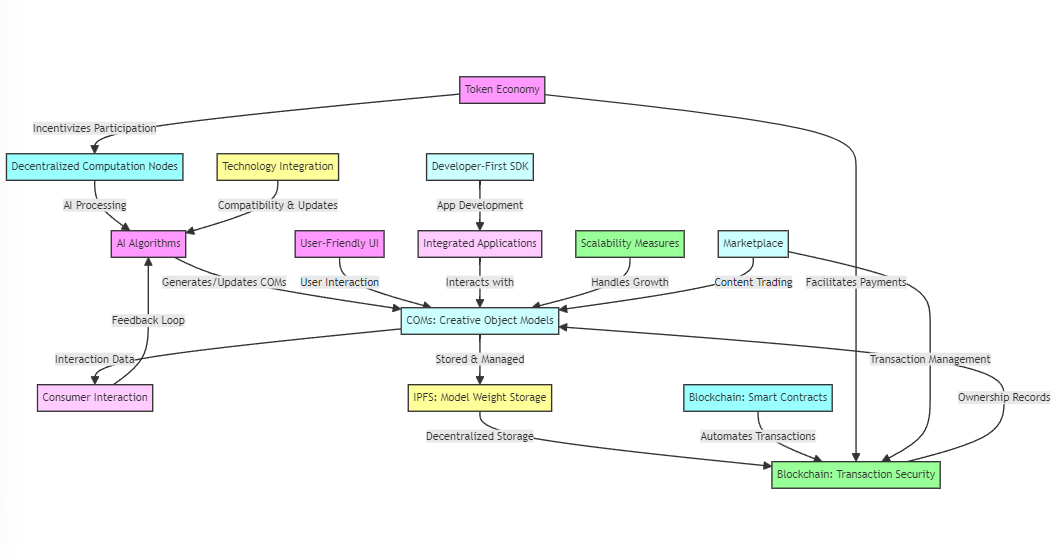
\includegraphics[width=1\linewidth]{create_4.png}
    \caption{High-level system architecture}
    \label{fig:system-architecture}
\end{figure}

\subsection{Integration with Existing and Emerging Technologies}

The Create protocol is designed to be interoperable with a range of existing and emerging technologies. This includes compatibility with various blockchain networks, integration with different AI and machine learning platforms, and adaptability to future technological advancements. Such integration ensures that the protocol remains at the forefront of the digital creative space, continuously evolving and improving its capabilities.

\subsection{Scalability and Future-Proofing the Protocol}

Understanding the dynamic nature of technology, the Create protocol is built with scalability and future-proofing in mind. The architecture is designed to handle increased loads and complexities as the user base and the scope of interactions grow. This ensures that the protocol can adapt and expand to meet future demands, maintaining its efficiency and effectiveness in the ever-evolving landscape of digital creativity.

\noindent\fbox{%
    \parbox{\textwidth}{%
To summarize, the "Technology and Infrastructure" section of the whitepaper offers a thorough examination of the advanced technological framework that forms the basis of the Create protocol. It emphasizes the incorporation of artificial intelligence, blockchain technology, decentralized storage, and user-focused design, all collaborating to foster a dynamic, safe, and expandable environment for the digital creative economy.
}%
}

\pagebreak

\section{Governance and Tokenomics}

This section of the Create protocol whitepaper delves into the governance structure and tokenomic model that underpin the protocol ecosystem. These elements are crucial for maintaining a balanced, equitable, and sustainable platform, ensuring that it adapts to changing needs while aligning the interests of all stakeholders - artists, consumers, computation nodes, and platform administrators.

\subsection{Distribution of Governance Tokens}

The Create protocol employs a governance token system to facilitate decentralized decision-making. The tokens represent voting power and are distributed among key stakeholders to ensure a democratic and fair governance process.

\begin{itemize}
    \item \textbf{Admins}: This group includes the protocol's founders and key developers. Their allocation reflects their ongoing role in maintaining and upgrading the platform.
    \item \textbf{Artists}: Recognizing the central role of creators in the ecosystem, a significant portion of governance tokens is allocated to artists. This ensures they have substantial influence over decisions that affect the platform's creative direction.
    \item \textbf{Computation Nodes}: These stakeholders provide the computational power necessary for the AI-driven personalization of COMs. Their allocation allows them to have a say in technical and operational aspects of the platform.
\end{itemize}

\subsection{Roles and Responsibilities in Governance}

The governance model is designed to balance different interests and perspectives:

Admins are responsible for proposing and implementing technical updates, security measures, and overall platform improvements.
Artists influence decisions related to creative policies, royalty structures, and community guidelines.
Computation nodes contribute to decisions regarding infrastructure, scalability, and technical optimizations.

\subsection{Voting and Decision-Making Processes}

Decisions within the Create protocol are made through a transparent voting process, where stakeholders use their governance tokens to vote on proposals. This process ensures that changes to the protocol, such as updates to the royalty formula or modifications to the AI algorithms, are made democratically and reflect the collective interest of the community.

\subsection{Smart Contract Updates and Security Measures}

The protocol employs smart contracts for various functions, including royalty distribution, token transactions, and governance voting. Regular updates and audits of these smart contracts are essential for maintaining security and efficiency. The governance model allows for these updates to be proposed, reviewed, and implemented in a structured and secure manner.

\subsection{Tokenomic Model: Balancing Supply and Demand}

The tokenomic model of the Create protocol is carefully designed to balance supply and demand, ensuring long-term sustainability. The \$CREATE token serves multiple purposes: it's used for transactions within the ecosystem, represents voting power in governance, and acts as an incentive for various stakeholders. Mechanisms such as token burning, rewards for participation, and controlled token release schedules are employed to maintain a healthy economic balance.

\subsection{Economic Incentives and Rewards System}

The protocol encourages active participation and contribution to the ecosystem. Artists are rewarded for creating and updating COMs, consumers are incentivized through unique content experiences, and computation nodes are compensated for providing computational resources. This rewards system ensures ongoing engagement and growth of the platform.

\subsection{Long-Term Governance and Economic Strategies}

The long-term vision for governance and economics within the Create protocol involves adaptive strategies that can respond to evolving market conditions, technological advancements, and community needs. This includes potential adjustments to token distribution, voting mechanisms, and economic incentives to ensure that the protocol remains relevant, vibrant, and equitable.

\noindent\fbox{%
    \parbox{\textwidth}{%
To sum up, the section titled "Governance and Tokenomics" in the whitepaper presents a thorough structure for decentralized decision-making and a well-balanced economic model. The aim of this structure is to give authority to stakeholders, ensure the integrity of the platform, and promote a sustainable and prosperous ecosystem for the future of digital creativity.}%
}

\pagebreak

\section{Use Cases of COM}

This portion of the whitepaper on the Create protocol discusses the practical uses and real-life situations in which Creative Object Models (COMs) can be employed. It emphasizes the adaptability and game-changing possibilities of COMs in different fields, demonstrating how they can fundamentally change the manner in which we engage with digital content.

\subsection{Creative Applications Across Various Domains}

COMs, with their dynamic and interactive nature, have a wide array of applications in diverse creative fields:

\begin{itemize}
    \item \textbf{Digital Art and Design:} Artists can create evolving artworks that change over time or in response to viewer interactions, offering a unique, immersive experience that goes beyond traditional static art.
    \item \textbf{Music Production:} Musicians and producers can use COMs to create adaptive music tracks that evolve based on listener preferences or environmental factors, such as time of day or weather.
    \item \textbf{Film and Animation:} Filmmakers can employ COMs to produce interactive films where the storyline or visual elements change based on viewer choices, creating a personalized viewing experience.
    \item \textbf{Fashion and Wearables:} Designers can leverage COMs to create digital fashion items that change styles, colors, or patterns, aligning with user preferences or trends.
\end{itemize}

\subsection{Example Scenarios: Blog Writing, Code Generation, and More}

Specific examples of COM usage demonstrate their potential to transform various industries:

\begin{itemize}
    \item \textbf{Blog Writing:} A COM has the ability to be trained using the style and expertise of a specific writer. This allows it to create personalized blog posts for various audiences, as desired by the end user. Just imagine having your blog post written by the renowned author, Hemmingway.
    \item \textbf{Code Generation:}COMs can be utilized by software developers to write code in a particular programmer's style or to automatically generate code snippets for specific tasks, thereby enhancing efficiency and ensuring consistency. Consider the scenario where you have the opportunity to have John Carmack, renowned for his work on Doom, write code according to your requirements.
    \item \textbf{Educational Content:}Computational objects (COMs) have the potential to generate interactive educational resources that can adjust to the individual learning speed and preferences of students, offering a personalized educational journey. Consider the scenario where Richard Feynman delivers a Quantum Computation lecture, incorporating his unique teaching style.
\end{itemize}

\subsection{Personalized Digital Interactions}

The unique selling point of COMs is their ability to facilitate personalized digital interactions. This personalization extends beyond mere content consumption, enabling users to interact with digital content that is responsive and adaptive to their individual preferences, behaviors, and feedback.

\subsection{Collaborative Art and Community Projects}

COMs also have the potential to foster collaborative art and community-driven projects. Artists and creators from around the world can contribute to a shared COM, resulting in a collective piece of art that is greater than the sum of its parts.

\subsection{Decentralized Content Creation and Distribution}

COMs enable a decentralized approach to content creation and distribution, empowering creators to retain control over their work, style, image and voice while engaging directly with their audience. This model disrupts traditional content distribution channels, democratizing content creation and access.

\subsection{Bridging the Gap Between Virtual and Physical Worlds}

Ultimately, COMs possess the capability to connect the divide between virtual and physical realms, generating encounters that go beyond the boundaries of the digital domain. This encompasses augmented reality encounters, interactions within virtual worlds, and various other applications within mixed reality.

\noindent\fbox{%
    \parbox{\textwidth}{%
To sum up, the section titled "Use Cases of COM" in the whitepaper demonstrates the extensive possibilities of COMs in transforming the digital creative field. By improving artistic expression and revolutionizing how content is consumed and interacted with, COMs provide a glimpse into a future where personalized experiences are created through the fusion of creativity and technology.
}%
}

\pagebreak

\section{Community and Ecosystem}

The "Community and Ecosystem" section of the Create protocol whitepaper is dedicated to illustrating the vibrant and dynamic community that forms the backbone of the protocol, as well as the burgeoning ecosystem that surrounds it. This section outlines how the protocol not only fosters a strong sense of community among its users but also actively contributes to the broader ecosystem of digital creativity and blockchain technology.

\subsection{Building a Collaborative Community of Artists, Developers, and Users}

At the heart of the Create protocol is a community ethos that champions collaboration, innovation, and shared growth. The protocol nurtures a diverse and inclusive community where artists, developers, and users converge to explore the vast possibilities of AI-driven creativity. This community is a melting pot of ideas, cultures, and talents, where members inspire and elevate each other, creating a rich tapestry of artistic and technological innovation.

\textbf{Artists and Creators:} The protocol empowers artists by providing them with tools to express their creativity in novel ways, protect their intellectual property, and monetize their work in the evolving digital landscape.
\textbf{Developers and Technologists:} For developers, the protocol provides an excellent opportunity to create innovative applications, explore the possibilities of Generative AI technology, and avoid concerns about infringing on artists' copyrights while utilizing decentralized computation as needed.
\textbf{Users and Consumers:} Users are integral to the community, providing valuable feedback, participating in governance, and shaping the future direction of the protocol through their interactions and preferences.

\subsection{Fostering Collaborative Opportunities and Ecosystem Growth}

The Create protocol promotes a culture of collaboration and shared development. It enables artists and technologists to form partnerships, opening doors for collaborative projects, interdisciplinary initiatives, and joint creation. These collaborations have a ripple effect, reaching beyond the protocol and influencing the larger creative and technology communities.
\subsection{Engaging with the Broader Creative and Tech Communities}

The protocol's community engagement strategy involves outreach to broader creative and technological circles. This includes participating in industry events, forming alliances with art collectives and tech consortia, and contributing to open-source projects. By engaging with these communities, the protocol not only gains visibility but also infuses fresh perspectives and ideas into its ecosystem.

\subsection{Educational Initiatives and Resource Sharing}

Understanding the importance of education and knowledge sharing, the Create protocol invests in educational initiatives aimed at both novices and experts. These initiatives include online workshops, webinars, tutorials, and resource libraries that cover topics from basic blockchain technology to advanced AI-driven creative processes. This educational thrust ensures that the community remains at the forefront of technological and creative advancements.

\subsection{Championing Openness and Transparency}

The protocol’s commitment to openness and transparency is a cornerstone of its community philosophy. This includes maintaining open channels of communication, publishing transparent reports on developments and decisions, and actively seeking community feedback. Such transparency fosters trust and strengthens the bond between different stakeholders in the ecosystem.

\subsection{Sustaining a Dynamic and Evolving Ecosystem}

The long-term vision for the Create protocol’s community and ecosystem is one of sustained dynamism and evolution. This vision is realized through ongoing community engagement, adaptation to technological advancements, and responsiveness to the ever-changing landscape of digital creativity.

\noindent\fbox{%
    \parbox{\textwidth}{%
To sum up, the "Community and Ecosystem" section of the whitepaper presents a captivating story of a flourishing and interconnected community as the foundation of the Create protocol. It depicts an ecosystem that is not only strong and inventive, but also welcoming and cooperative, fueled by a common enthusiasm for reshaping the limits of digital creativity and blockchain technology. This section emphasizes the protocol's dedication to fostering a community that is essential to its identity and pivotal to its achievements.}%
}

\pagebreak

\section{Future Roadmap and Development Plans}

The section titled "Future Roadmap and Development Plans" in the Create protocol whitepaper presents a strategic and progressive plan for the protocol's development and expansion. This roadmap aims to steer the protocol through different stages of growth, initially concentrating on text and images and later progressing to more intricate forms of media such as video and audio. It demonstrates a well-defined and ambitious vision for the future, characterized by gradual progress and scalability.

\subsection{Initial Focus: Text and Images}

\subsubsection{Phase 1: Text-Based COMs}

The first stage of the Create protocol will prioritize the development of text-based Creative Object Models (COMs). These COMs will provide writers, bloggers, and content creators with tools and platforms to produce dynamic written content that is enhanced by AI. The main goal is to create a non-copyrighted base mode, QLora finetuning, and inference infrastructure for an Open Source LLM. This LLM will have the ability to imitate various writing styles, adjust content based on the input provided by artists, and generate personalized written content.

\subsubsection{Phase 2: Image-Based COMs}

After the successful integration of text-based COMs, the protocol will be extended to incorporate image-based COMs, with the aim of applying the same approach to diffusion models. This stage will specifically cater to the needs of digital artists, graphic designers, and photographers. The main focus will be on developing tools that enable the creation, personalization, and interactive development of digital images and artworks.


\subsection{Expansion to Video and Audio}


\begin{figure}
    \centering
    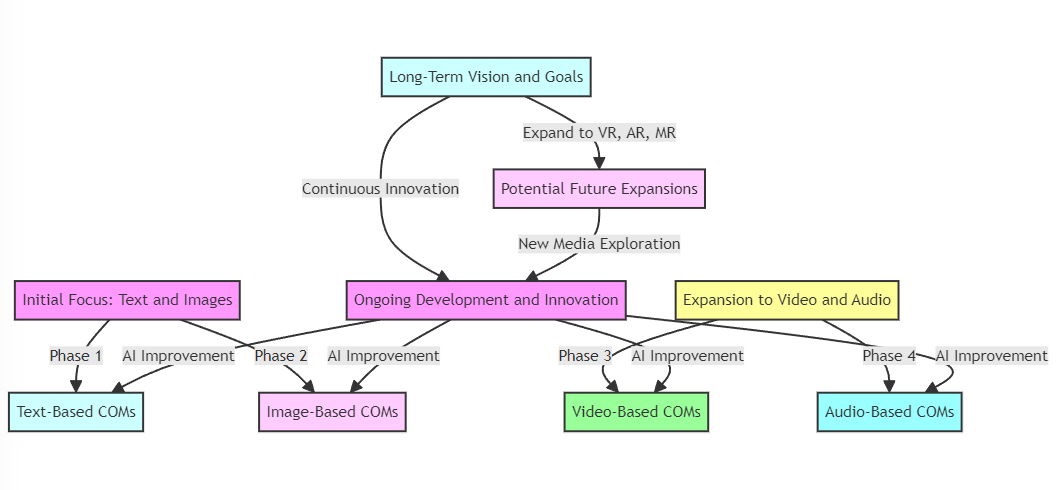
\includegraphics[width=1\linewidth]{create_5.png}
    \caption{Roadmap}
    \label{fig:roadmap}
\end{figure}

\subsubsection{Phase 3: Video-Based COMs}

AAs the protocol evolves, the next stage will involve incorporating video-based communication methods. This phase will focus on catering to filmmakers, animators, and creators of video content by equipping them with tools to generate dynamic video content enhanced by artificial intelligence. The primary objectives for this phase of development will encompass advanced video editing and production tools driven by AI, algorithms with the ability to comprehend and adapt to narrative structures, as well as interactive capabilities enabling viewers to impact video content.
\subsubsection{Phase 4: Audio-Based COMs}

The forthcoming expansion will involve the inclusion of audio-based communication systems, with a specific focus on musicians, podcasters, and producers of audio content. The objective of this phase is to bring about a significant transformation in the way audio content is generated, distributed, and consumed. This will be achieved by utilizing artificial intelligence (AI) to create adaptive and personalized audio experiences. The development efforts in this phase will primarily concentrate on the advancement of audio processing technologies, AI-powered tools for music composition, and interactive audio systems that can adapt to the preferences and feedback of listeners.

\subsection{Ongoing Development and Innovation}

During all stages, there will be a consistent focus on improving the AI algorithms, enhancing user interfaces, and guaranteeing the scalability and security of the platform. The protocol will also remain flexible to new technologies and market trends, ensuring it remains at the forefront of the digital creative field. The input and participation of the community will be vital in directing the development process. Regular updates, beta testing with community members, and open forums for feedback will ensure that the protocol progresses in accordance with the needs and preferences of its users.

\subsection{Long-Term Vision and Goals}

The Create protocol has a grand vision of creating a platform that is comprehensive, adaptable, and easy to use, catering to a diverse range of creative expressions in different media. The objective is to become a prominent player in the AI-driven creative industry, renowned for its cutting-edge ideas, high standards, and active community involvement. The protocol intends to consistently push boundaries in digital creativity, with potential future expansions into emerging areas like virtual reality (VR), augmented reality (AR), and mixed reality (MR) experiences.

\noindent\fbox{%
    \parbox{\textwidth}{%
To summarize, the "Future Roadmap and Development Plans" section of the whitepaper outlines a well-defined and ambitious plan for the advancement of the Create protocol. It exhibits a dedication to continuous progress, beginning with basic content such as text and images, and gradually expanding to include more intricate forms of media like video and audio. This roadmap signifies a vision of a platform that is both technologically advanced and adaptable, prioritizing user needs and adapting to the ever-changing digital creative environment.}%
}

\pagebreak

\section{Summary}

As we reach the culmination of this whitepaper, it is clear that the Create protocol represents more than just a technological innovation; it is a call to action, an invitation to be part of a groundbreaking movement in the realm of digital creativity. The vision outlined in these pages is ambitious, transformative, and achievable - but only with the collective effort and passion of a diverse community of creators, developers, users, and visionaries.

The Create protocol is not just a platform; it's a catalyst for unleashing the full potential of creative expression in the AI era. It's an ecosystem where each participant has the power to contribute, innovate, and be part of something that is much larger than themselves. This is a unique opportunity to be at the forefront of a revolution, to shape the future of digital creativity, and to be part of a community that is redefining the boundaries of what is possible.

\subsection*{The Call to 100x Contribution and Impact}

\textit{For Artists and Creators:} This is your canvas to redefine art and creativity. Your participation in the Create protocol is not just about showcasing your work; it's about amplifying your creative impact a hundredfold. By contributing to this platform, you are not just creating; you are inspiring, influencing, and leading a new wave of digital artistry.

\textit{For Developers and Technologists:} Your skills and ingenuity have the power to drive this platform to new heights. The Create protocol is a sandbox for innovation, where your code can breathe life into unprecedented forms of creative expression. Your contribution is the bridge between artistic vision and technological breakthrough.

\textit{For Users and Consumers:} You are the lifeblood of the Create protocol. Your interactions, feedback, and engagement are what will shape the platform and its content. By being part of this community, you have the power to personalize your digital experience, influence creative trends, and be an active participant in a creative revolution.

\textit{For Visionaries and Thought Leaders:} Your insights, foresight, and guidance are crucial in steering the Create protocol towards its full potential. Your involvement will help to nurture a vibrant community, foster innovative ideas, and ensure that the protocol remains at the cutting edge of technology and creativity.

\subsection*{Embracing the 100x Mindset}

The Create protocol is more than just a technological marvel; it's a mindset. It's about thinking bigger, pushing boundaries, and striving for exponential impact. Whether you are an artist, developer, user, or visionary, you are an integral part of this journey. Together, as a united community, the potential for growth, innovation, and creativity is limitless. We can achieve 100 times more than what we can imagine individually.

\subsection*{Join Us in Shaping the Future}

As we look to the future, the Create protocol stands as a beacon of potential and promise. It's a journey that we embark on together, each of us playing a crucial role in shaping the landscape of digital creativity. We invite you to join us in this exciting endeavor. Contribute your art, your skills, your ideas, and your passion. Be part of a community that is not just witnessing the future but actively creating it.

To summarize, the Create protocol offers a platform for individuals to discover, experiment, and revolutionize the realm of digital creativity. Join this movement and accept the opportunity to contribute, cooperate, and bring about the transformation you desire. Let's come together to enhance the digital world, making it a more vibrant, dynamic, and imaginative space. Together, we can all achieve greatness.

\end{document}